\documentclass[onecolumn, draftclsnofoot,10pt, compsoc]{IEEEtran}
\usepackage{graphicx}
\usepackage{url}
\usepackage{setspace}

\usepackage{geometry}
\geometry{textheight=9.5in, textwidth=7in}

% 1. Fill in these details
\def \CapstoneTeamName{		ConnectBasket Development Team}
\def \CapstoneTeamNumber{		39}
\def \GroupMemberOne{			Henry Fowler}
\def \GroupMemberTwo{			Kailyn Hellwege}
\def \GroupMemberThree{			Taylor Kirkpatrick}
\def \CapstoneProjectName{		ConnectBasket}
\def \CapstoneSponsorCompany{	OSU MIME}
\def \CapstoneSponsorPerson{		C Eseonu}

% 2. Uncomment the appropriate line below so that the document type works
\def \DocType{		%Problem Statement
				Requirements Document
				%Technology Review
				%Design Document
				%Progress Report
				}
			
\newcommand{\NameSigPair}[1]{\par
\makebox[2.75in][r]{#1} \hfil 	\makebox[3.25in]{\makebox[2.25in]{\hrulefill} \hfill		\makebox[.75in]{\hrulefill}}
\par\vspace{-12pt} \textit{\tiny\noindent
\makebox[2.75in]{} \hfil		\makebox[3.25in]{\makebox[2.25in][r]{Signature} \hfill	\makebox[.75in][r]{Date}}}}
% 3. If the document is not to be signed, uncomment the RENEWcommand below
\renewcommand{\NameSigPair}[1]{#1}

%%%%%%%%%%%%%%%%%%%%%%%%%%%%%%%%%%%%%%%
\begin{document}
\begin{titlepage}
    \pagenumbering{gobble}
    \begin{singlespace}
    	
\includegraphics[height=4cm]{coe_v_spot1}
        \hfill 
        % 4. If you have a logo, use this includegraphics command to put it on the coversheet.
        %\includegraphics[height=4cm]{CompanyLogo}   
        \par\vspace{.2in}
        \centering
        \scshape{
            \huge CS Capstone \DocType \par
            {\large\today}\par
            \vspace{.5in}
            \textbf{\Huge\CapstoneProjectName}\par
            \vfill
            {\large Prepared for}\par
            \Huge \CapstoneSponsorCompany\par
            \vspace{5pt}
            {\Large\NameSigPair{\CapstoneSponsorPerson}\par}
            {\large Prepared by }\par
            Group\CapstoneTeamNumber\par
            % 5. comment out the line below this one if you do not wish to name your team
            \CapstoneTeamName\par 
            \vspace{5pt}
            {\Large
                \NameSigPair{\GroupMemberOne}\par
                \NameSigPair{\GroupMemberTwo}\par
                \NameSigPair{\GroupMemberThree}\par
            }
            \vspace{20pt}
        }
        \begin{abstract}
        % 6. Fill in your abstract    
        This document describes in detail the requirements for the ConnectBasket development team for 2017-2018. The document will describe the purpose and scope of the project as well as describing the users that will interact with the finished project. It will describe in detail each of the specific requirements as well as some additional stretch goals to be completed if there is time.
        \end{abstract}     
    \end{singlespace}
\end{titlepage}
\newpage
\pagenumbering{arabic}
\tableofcontents
% 7. uncomment this (if applicable). Consider adding a page break.
%\listoffigures
%\listoftables
\clearpage

% 8. now you write!
\section{Introduction}

\subsection{Purpose}
The purpose of this document is to outline the requirements for an improved communication system for the Oregon State University (OSU) Veterinary Hospital, called ConnectBasket. 
This document's audience is the client, as well as certain staff members at the hospital. This document will be used as a way to measure the success of the Capstone development team working on this project. 


\subsection{Scope}
ConnectBasket will be an electronic system for the OSU Veterinary Hospital that will streamline the way messages are moved around the hospital and provide a better way to track the route that messages have taken. When an owner calls the hospital, receptionists will be able to type a message into the computer, assign it a category, and route it to the necessary staff members, which may be service specific vet techs, house officers, or faculty. Those staff members will be alerted, either by email or text, that they have a message waiting for them in ConnectBasket, and once viewed, notes can be added and the message can be re-routed to other staff members. After a message has been addressed by the necessary staff, the message can be closed, meaning no more notes can be added. The audit trail of when the message was created and closed will be visible, along with all the notes, timestamps of notes, and staff who added the notes.


\subsection{Definitions, Acronyms, and Abbreviations}
Capstone - CS 461 class at Oregon State that the developers of ConnectBasket are in 
OSU - Oregon State University
Hospital - referring to the OSU Veterinary Hospital
Owner - a person who owns a pet that is a client of the hospital
Patient - an animal who has/is going to be treated at the hospital 
VetHosp - the hospital management system used by the OSU Veterinary Hospital for keeping patient and owner records
Mobile Devices - smartphones or tablets
Workflow - a process in which tasks or assignments are started, worked on, and completed

\subsection{References}
IEEE Std 830-1998, IEEE Recommended Practice for Software Requirements Specifications

\subsection{Overview}
The second section of this document will contain a further description of the ConnectBasket project, including product functions, user characteristics, and constraints. The third section will define the specific requirements of the project. 

\section{Overall Description}

\subsection{Product Perspective}
The ConnectBasket software system will be a stand alone system that will have additional functionality to connect to the current VetHosp system used by the hospital. ConnectBasket will use patient and owner information stored in the VetHosp system to connect information collected with the correct patients and owners.

\subsubsection{User Interfaces}
There will need to be some level of security requiring users to login to access the information in the system. The system will provide users with the ability to search for a patient or owner and to enter new messages for them as well as view older messages and the audit trail associated with the message.

\subsubsection{Hardware Interfaces}
Users will access the system from their mobile devices or desktop computers. The system will need to communicate with a server at the hospital that has information about patients and owners stored in a database.

\subsubsection{Software Interfaces}
ConnectBasket must be able to interface with the VetHosp program in order to connect information collected with the information about patients and owners stored in VetHosp.

\subsection{Product Functions}
ConnectBasket will allow users to create messages associated with patients and owners of the hospital. They will then be able to route that message to one or more staff members, who will then be able to add to that message and route it elsewhere if necessary. When all necessary actions have been taken, a message can be flagged as completed, and users with appropriate permissions will be able to view an audit log of the message.

\subsection{User Characteristics}
Users of ConnectBasket will be staff members of the hospital. The users will have a variety of different education levels and experience. Therefore, the system will need by designed so that technical expertise is not required in order to properly use it.

\subsection{Constraints}
The performance of the ConnectBasket application will be limited by a staff member's internet connection. Staff should not use the service on unsecure networks, as messages sent with it should have some degree of confidentiality due to the nature of the work, the hospital's policies, and government regulations. This limits where the application can be accessed from, as non-trusted networks may expose these messages. Staff may also only access this application with a verified user account to use these features.

\subsection{Assumptions and Dependencies}
It will be assumed that staff will not be attempting to use non-English languages for messaging. This system will depend on the hospital's existing VetHosp software, and integration with it is a goal for this project. Integration will depend on the VetHosp software being available to the developers and the level of access the development team will have to it. VetHosp integration will also depend on the hospital's IT team arranging an integration of ConnectBasket with VetHosp.

\section{Specific Requirements}

\subsection{External interface requirements}

\subsubsection{VetHosp}
ConnectBasket will be integrated with VetHosp as it nears completion, so that it can pull information from VetHosp as needed to populate fields and reduce separate instances of data lookup. Detailed info about VetHosp is not currently available to the development team, but more information should be available later on.

\subsection{System features}

\subsubsection{Creation of Messages}
ConnectBasket shall allow receptionists to create messages and route them to other parts of the hospital. Receptionists and other staff should be able to route messages with patient information to the relevant locations in the hospital. These messages should be secure and not exposed to public channels, and may need to be encrypted as well.

\subsubsection{Message Auto Population}
ConnectBasket shall allow message composers to easily write messages by auto populating some fields of the message, such as the current date and patient and owner names. By auto filling and not allowing free text for certain fields, message creation will be more efficient and less error-prone. These fields will be prefilled for convenience and to send off messages quicker and in a standard format. This feature will also include utilizing drop-down menus instead of plain text to reduce error for other fields, such as recipients of messages and category of messages.

This feature was specifically mentioned by the client as a high priority feature. It is important and will be useful for both convenience and safety, as constraining messages to at least some pre-defined standard will reduce the likelihood of human error in medical situations.

\subsubsection{Message Notification}
ConnectBasket shall send message recipients notifications should they receive messages. Notifications shall be delivered as a text message, email, or both, depending on the preferences of the staff member. Staff members will have the option to receive alerts simply after a message is received or after a message is unread for a portion of time.

\subsubsection{Message Review and Forwarding}
ConnectBasket shall allow message recipients to review their messages online via any internet-accessible device, should the connection or other factors not restrict them from doing so. Staff who have viewed a message shall be capable of rerouting this same message to other necessary staff, along with any comments or addendums added by the previous recipient. 

This feature is a baseline expected feature that one would expect in any messaging software. This is also essential in a hospital environment due to the nature of the work and how frequently detailed communication between a large number of people must take place.

\subsubsection{Message Resolution}
ConnectBasket shall allow message recipients to resolve messages as closed, should the task or job mentioned within it be completed. This closed state should remove the message from all staff member's queues, allowing them to focus on other tasks that have not been resolved.
	
The ability to resolve tasks and mark tasks as complete is essential to any workflow. Ideally, this feature will include more than just a closed state; it will also include additional states that show other reasons for a task to no longer be active, such as cancelled, duplicate, or stopped, to provide more information about the status of a task.

\subsubsection{Message Audit Record}
ConnectBasket shall allow staff with sufficient permissions to view a message's  history for audit or review. Authorized staff will  be able to see when and where the message was created, when and where it was routed, and when and where it was closed. The name of any staff member who took any action should also be recorded, along with other activity regarding a message. 

Providing an audit trail for all messages will provide the hospital with valuable information and allow them to track metrics such as the average amount of time the hospital takes to respond to calls and common reasons for owners calling the hospital. 

\subsubsection{Message Recipient Roles and Profile Roles}
ConnectBasket shall allow users to select and be assigned to one or more roles that reflect their duties and responsibilities at the hospital. Staff will have profiles to manage their roles, with the ability to change their roles at will. When messages are routed to a specific department, any staff member that has selected the associated role to that department will receive the message in a queue accessible by anyone assigned to the role. These staff members will be able to take ownership of the message to interact with it, or interact with it to a lesser degree without taking ownership of the message. All of the regular message features that are accessible to individual staff members will also be accessible to the all the staff members that receive a message in a role. 

This feature is also a staple of any quality workflow manager, and should be vital in a hospital setting or any setting where the staff is large enough. Staff in one location can not assume, and should not have to assume, whether a certain employee is available or whether a task falls under their responsibilities. Assigning messages to a role and putting them in queues removes the necessity for staff to understand structure in other departments, and allows tasks and messages to be passed faster and with less room for error.

\subsection{Performance Requirements}

\subsubsection{Web Service}
As ConnectBasket needs to be accessible from most internet accessible devices, it must be a web application. Native applications are an option, but this would require a significant amount of extra work in customizing an application for Windows, Mac, Android, iOS, among other systems. A web application is more reasonable in the timeframe of the senior capstone project because it can be used on a variety of devices as well as scaled to different sized devices.

This web application will need to be accessible from any internet accessible device. Staff will be doing vital work through this application, and so it must be accessible to them, no matter what device they have. However, there are constraints on how accessible this is. Internal messaging must remain confidential and secure, and staff should have secure profiles to restrict access to malicious persons. ConnectBasket must be reliable and have minimal downtime, as this application going down could cripple the work of the hospital staff once it is deployed. Downtime should be kept to a maximum of two hours a week once in a fully completed state. Two hours per week allows for security patching and maintenance should it be required, though this number may change depending on the specific processes as they are defined.

\subsection{Design Constraints}
ConnectBasket will be constrained only by any government or hospital regulations on message security or reliability. Regulations may require audit trails or set a maximum downtime for the application, which will restrict the design as these come to light.

In addition, while not a mandatory constraint, eventual integration with VetHosp is the long term goal for this project. If the project is built in such a way as to ease the connection between the two, this design choice may save a significant amount of time. However, with a lack of knowledge about VetHosp, designing in such a way is unlikely and thus, not a mandatory element of the design.
\newpage
\section{Appendix I: Gantt Chart}
Note that the following Gantt chart is only a basic outline on the high-level plan for the ConnectBasket development period. It is subject to change at any time and should not be referenced for specific deadlines.

Also note that the date of Expo is not final, and is only assumed to be that date because of last year's schedule.

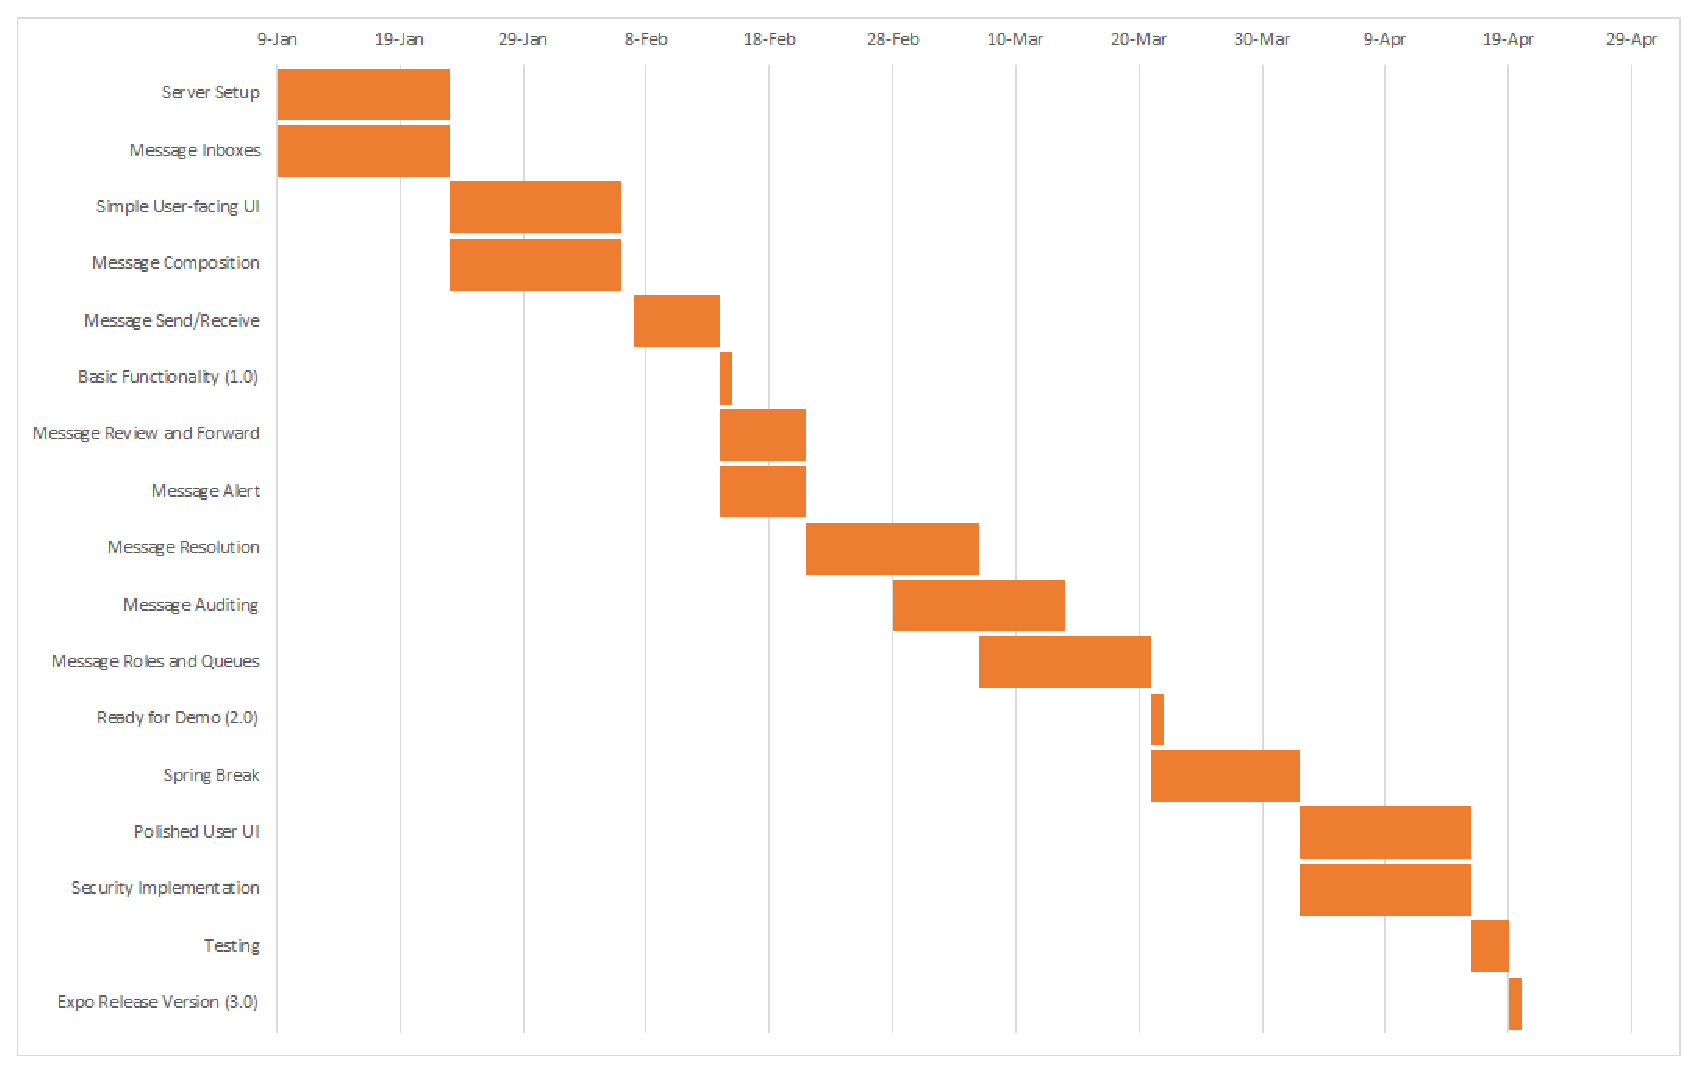
\includegraphics[angle=-90,origin=c,width=\textwidth,height=\textheight,keepaspectratio]{gantt-chart.eps}

\end{document}
